% 第 17 题三棱台图：按固定源 PDF 矢量路径换算（1 pt → 0.03515 cm）。
% 原点取顶点 A（源页 (980.7578, 532.9297) pt），y 向上。
% 顶点：A(0,0)、B(109.37,−41.43)、C(152.25,0)、D(65.52,37.58)、E(118.04,21.68)、F(143.57,37.58)。
% 实线 8 段（含题图额外画出的 BF——题干要求证 BF⊥平面 ACFD）；虚线 1 段：AC（被遮挡的底棱）。无箭头。
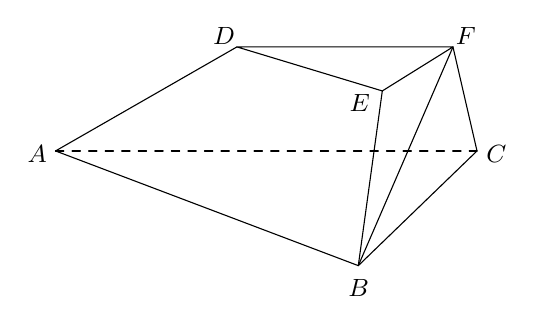
\begin{tikzpicture}[line cap=round,line join=round,font=\small,x=0.03515cm,y=0.03515cm]
% ===== 虚线先画（底棱 AC）=====
\draw[dash pattern=on 2.99pt off 2.99pt] (0,0)--(152.25,0);
% ===== 实线 =====
\draw (109.37,-41.43)--(0,0);        % BA
\draw (109.37,-41.43)--(152.25,0);   % BC
\draw (65.52,37.58)--(0,0);          % DA
\draw (118.04,21.68)--(109.37,-41.43); % EB
\draw (143.57,37.58)--(152.25,0);    % FC
\draw (109.37,-41.43)--(143.57,37.58); % BF（题图额外线段）
\draw (118.04,21.68)--(143.57,37.58)--(65.52,37.58)--cycle; % 上底 DEF（EF、FD、DE）
% ===== 标注（照源字形框中心，显式坐标）=====
\node[anchor=center,inner sep=0] at (-6.60,-1.06) {\(A\)};
\node[anchor=center,inner sep=0] at (109.52,-49.49) {\(B\)};
\node[anchor=center,inner sep=0] at (159.27,-1.06) {\(C\)};
\node[anchor=center,inner sep=0] at (60.84,41.46) {\(D\)};
\node[anchor=center,inner sep=0] at (109.87,17.20) {\(E\)};
\node[anchor=center,inner sep=0] at (148.20,41.46) {\(F\)};
\end{tikzpicture}
